\documentclass[twoside]{article}

\usepackage{amsmath,amsthm,amssymb,graphicx}
\usepackage{hyperref}
\usepackage[numbers]{natbib}
\usepackage{float}

\theoremstyle{definition}
\newtheorem{thm}{Theorem}[section]
\newtheorem{lem}[thm]{Lemma}
\newtheorem{prop}[thm]{Proposition}
\newtheorem{cor}[thm]{Corollary}
\newenvironment{pf}{{\noindent\sc Proof. }}{\qed}
\newenvironment{map}{\[\begin{array}{cccc}} {\end{array}\]}

\newcommand{\comment}[1]{}
\theoremstyle{definition}
\newtheorem*{defn}{Definition}
\newtheorem*{exmp}{Example}
\newtheorem*{prob}{Problem}

\theoremstyle{remark}
\newtheorem*{rem}{Remark}
\newtheorem*{note}{Note}
\newtheorem*{exer}{Exercise}

\setlength{\oddsidemargin}{0.25 in}
\setlength{\evensidemargin}{-0.25 in}
\setlength{\topmargin}{-0.6 in}
\setlength{\textwidth}{6.5 in}
\setlength{\textheight}{8.5 in}
\setlength{\headsep}{0.75 in}
\setlength{\parindent}{0 in}
\setlength{\parskip}{0.1 in}

\newcommand{\widgraph}[2]{\includegraphics[keepaspectratio,width=#1]{#2}}
\newcommand{\widgraphr}[3]{\includegraphics[keepaspectratio,width=#1,angle=#3]{#2}}

\newcommand{\lecture}[4]{
   \pagestyle{myheadings}
   \thispagestyle{plain}
   \newpage
   \setcounter{page}{1}
   \noindent
   \begin{center}
   \framebox{
      \vbox{\vspace{2mm}
    \hbox to 6.28in { {\bf cpsc 476/576 (Spring 2015) Computer Vision } }
       \vspace{6mm}
       \hbox to 6.28in { {\Large \hfill #1  \hfill} }
       \vspace{6mm}
       \hbox to 6.28in { {\it Name: #2 } }
      \vspace{2mm}}
   }
   \end{center}
   \markboth{#1}{#1}
   \vspace*{4mm}
}


%%%%%%%
% Some commonly used notation
%%%%%%%

\def\R{{\mathbb R}}
\def\X{{\mathcal X}}
\def\Y{{\mathcal Y}}
\def\H{{\mathcal H}}
\def\E{{\mathbb E}}
\def\sign{{\rm sign}}

\newcommand{\percent}{$\%$}

\begin{document}

\lecture{COMPUTER VISION - Homework 3}{Leon Lixing Yu}{Leon Lixing Yu}{1}

\section{Problem 1}
We have derived that the best fit line is given by
\[ \underset{W: \|W\|=1}{\operatorname{argmax}} \|X^T W\|^2\]
In which $W$ is the projection of $X$.
If we define the first singular vector $w_1$ of X as the best fit line for $X$ dataset. We will therefore have:
\[  w_1 = \underset{W: \|W\|=1}{\operatorname{argmax}} \|X^T W\|^2 \]
We also know that by SVD, 
\[ X = U\Sigma V^T \]
we can now write
\[  \underset{W: \|W\|=1}{\operatorname{argmax}} \|V\Sigma U^T W\|^2 = w_1\]
Becasue U and V are orthogonal matrices, they only rotate vectors without scaling them. We can then write
\[  \underset{W: \|W\|=1}{\operatorname{argmax}} \|V\Sigma U^T W\|^2 = \underset{W: \|W\|=1}{\operatorname{argmax}} \|\Sigma W\|^2 = w_1 \]
With the above equation proven, we know that $\Sigma$ is a diagonal matrix that are ordered from largest to smallest down the diagonal of itself. and $w_1$ is the best fit line for all possible $W$. If we put $U$, the orthogonal matrix from SVD back to the equation. We will have:
\[  \underset{W: \|W\|=1}{\operatorname{argmax}} \|\Sigma U^T W\|^2 = u_1 \]
Again since V only rotates the vectors, putting V back won't change the equation
\[  \underset{W: \|W\|=1}{\operatorname{argmax}} \|V \Sigma U^T W\|^2 = u_1 \]
\section{Problem 2}
The source code for problem 2 is included in the package. One can look for part2.m and pca.m to get the source code. The figure below illustrates the PCA given a dataset gaussian.mat.
\begin{figure}[H]
\centering
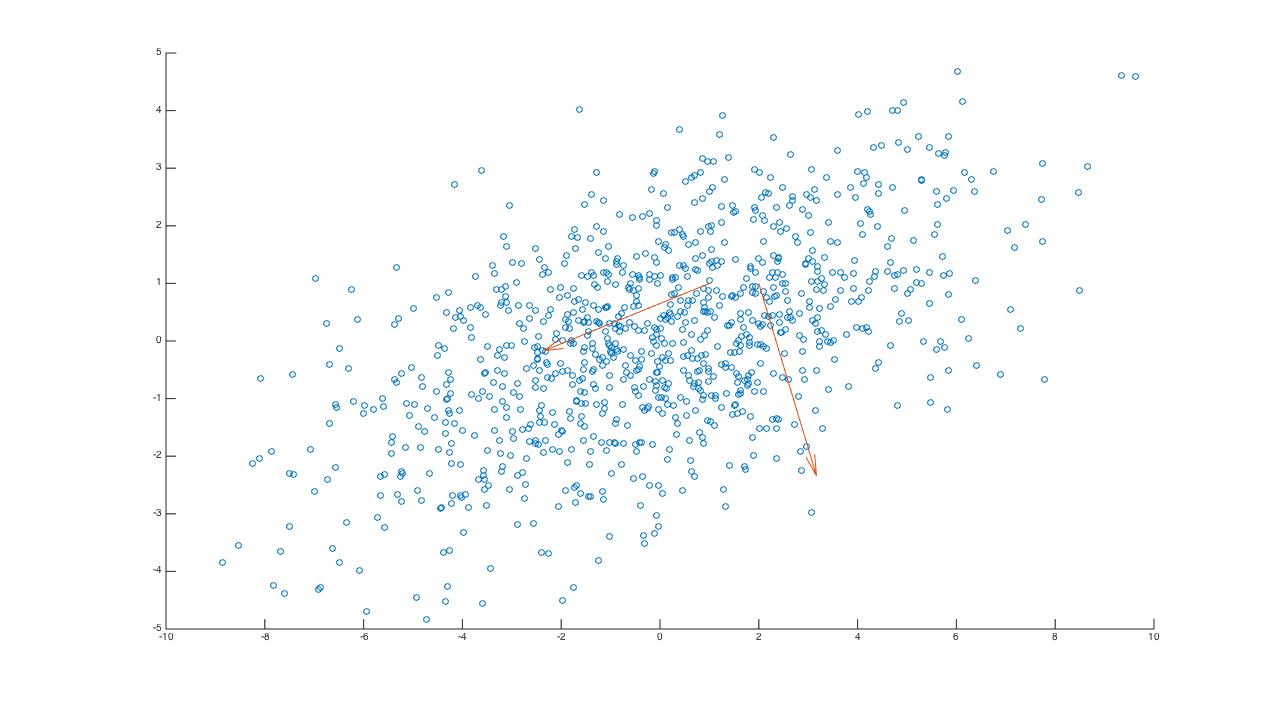
\includegraphics[width=120mm]{part2.jpg}
\caption{ pca on the dataset gassian.mat.  We can see that the first principle component lies alone the major axis of the data ellipse, and the 2nd PCA is orthogonal to the first components. Note that in order to make the PCAs visible, I scale the quiver plot by the norm of the variances \label{problem1Pic2}}
\end{figure}

\section{Problem 3}
The source code for problem 3 is included in the package. One can look for part3.m and diffmap.m to get the source code. The three figures below shows the diffmap function in action.
\begin{figure}[H]
\centering
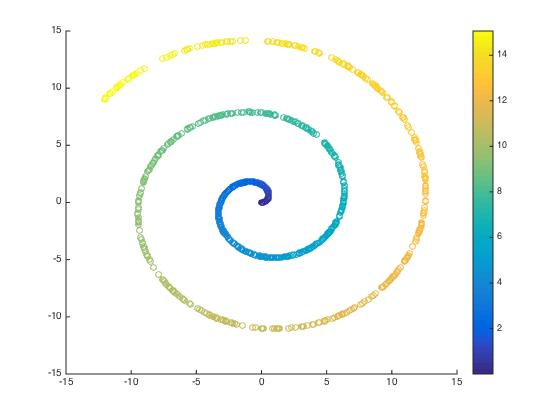
\includegraphics[width=120mm]{part3_1.jpg}
\caption{ A simple illustration of the spiral manifold dataset, meaning it is just a scatter plot of the data given. $Thetas$ indicates the position of each point along the spiral.  \label{problem1Pic2}}
\end{figure}

\begin{figure}[H]
\centering
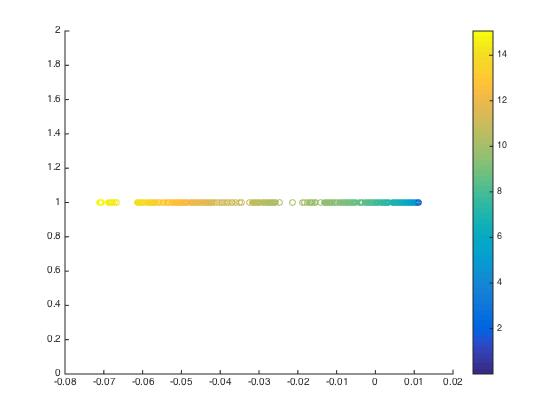
\includegraphics[width=120mm]{part3_2.jpg}
\caption{ 1st non-trivial coordinate function plotted alone X-axis while the Y-axis being a linspace. While using $Thetas$ as its color code, we can see that it matchs perfectly with the position of each point along the spiral. Note that the sign may be arbritary.  \label{problem1Pic2}}
\end{figure}

\begin{figure}[H]
\centering
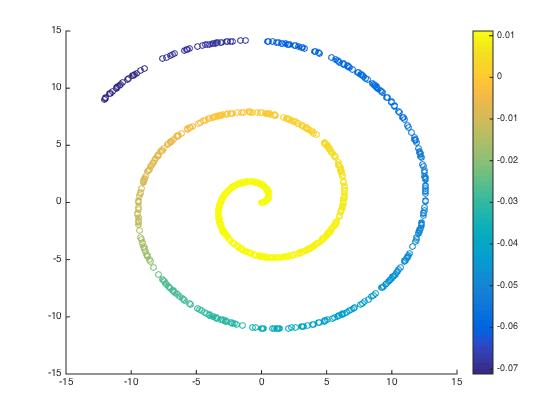
\includegraphics[width=120mm]{part3_3.jpg}
\caption{Spiral datset color-coded with the 1st non-trivial coordinate function, which indicates the distance range. We can clearly see that the the 1st non-trivial interpreted distance matches the $thetas$. \label{problem1Pic2}}
\end{figure}


\section{ Problem 4}
Since this problem is optional and potential final project option, I would like to leave it as one of my final project options. 







\end{document}
